\documentclass{article}

% if you need to pass options to natbib, use, e.g.:
% \PassOptionsToPackage{numbers, compress}{natbib}
% before loading nips_2018

% ready for submission
\usepackage[preprint]{nips_2018}


% to compile a preprint version, e.g., for submission to arXiv, add
% add the [preprint] option:
% \usepackage[preprint]{nips_2018}

% to compile a camera-ready version, add the [final] option, e.g.:
% \usepackage[final]{nips_2018}

% to avoid loading the natbib package, add option nonatbib:
% \usepackage[nonatbib]{nips_2018}

\usepackage[utf8]{inputenc} % allow utf-8 input
\usepackage[T1]{fontenc}    % use 8-bit T1 fonts
\usepackage{hyperref}       % hyperlinks
\hypersetup{colorlinks=true, citecolor=Blue, linkcolor=Brown}

\usepackage[capitalise,nameinlink]{cleveref}

\usepackage{url}            % simple URL typesetting
\usepackage{booktabs}       % professional-quality tables
\usepackage{amsfonts}       % blackboard math symbols
\usepackage{nicefrac}       % compact symbols for 1/2, etc.
\usepackage{microtype}      % microtypography
\usepackage{../am221}
\usepackage{algpseudocode,algorithm,algorithmicx}
\usepackage{bbm}
\usepackage{amsthm}

\newtheorem{theorem}{Theorem}

\linespread{1.1}
% \title{Formatting instructions for NIPS 2018}

% The \author macro works with any number of authors. There are two
% commands used to separate the names and addresses of multiple
% authors: \And and \AND.
%
% Using \And between authors leaves it to LaTeX to determine where to
% break the lines. Using \AND forces a line break at that point. So,
% if LaTeX puts 3 of 4 authors names on the first line, and the last
% on the second line, try using \AND instead of \And before the third
% author name.

% \author{
%   David S.~Hippocampus\thanks{Use footnote for providing further
%     information about author (webpage, alternative
%     address)---\emph{not} for acknowledging funding agencies.} \\
%   Department of Computer Science\\
%   Cranberry-Lemon University\\
%   Pittsburgh, PA 15213 \\
%   \texttt{hippo@cs.cranberry-lemon.edu} \\
%   %% examples of more authors
%   %% \And
%   %% Coauthor \\
%   %% Affiliation \\
%   %% Address \\
%   %% \texttt{email} \\
%   %% \AND
%   %% Coauthor \\
%   %% Affiliation \\
%   %% Address \\
%   %% \texttt{email} \\
%   %% \And
%   %% Coauthor \\
%   %% Affiliation \\
%   %% Address \\
%   %% \texttt{email} \\
%   %% \And
%   %% Coauthor \\
%   %% Affiliation \\
%   %% Address \\
%   %% \texttt{email} \\
% }

% Commands
\renewcommand{\b}{\mathbf}
\newcommand{\R}{\mathbb{R}}
\newcommand{\one}{\mathbbm{1}}
\newcommand{\E}{\mathbb{E}}

\newcommand{\KL}{\operatorname{KL}}
% Thm definitions
\theoremstyle{definition}
\newtheorem{prop}{Proposition}
\theoremstyle{remark}
\newtheorem{rmk}{Remark}

\title{Let's Get Movin': Frontiers of Optimal Transport}
\author{Jiafeng Chen\\School of Engineering and Applied Sciences\\Harvard University\\\url{jiafengchen@college.harvard.edu}\And Francisco Rivera\\School of Engineering and Applied Sciences\\Harvard University\\\url{frivera@college.harvard.edu}}
\date{\today}

\newcommand{\feasible}{\b U(\b a, \b b)}

\begin{document}
\maketitle
\section{Introduction and Background}

This project should serve as an introductory note and broad overview of both
 theoretical and computational aspects of the
 optimal transport literature. We hope that this note demonstrates both the
 theoretical elegance and practical versatility of optimal transport
 problems, and we hope to bring the reader to the forefront of the
 literature by going through a few recent articles in detail.

The organization of this report is as follows: \cref{sub:problem_intro}
introduces the discrete optimal transport problem and discusses its
interpration, dual problem, and basic theoretical properties as a linear
program. \cref{sec:exact} discusses methods to solve the optimal transport
problem \eqref{eq:ot_problem} exactly, introducing the Hungarian algorithm
\cite{kuhn2010hungarian} in \cref{sub:hungarian_algorithm} and presenting an
empirical analysis of its runtime. The Hungarian algorithm appears cubic in
run-time, confirming theoretical asymptotic analysis, which is optimal for exact
solution of \eqref{eq:ot_problem}, but is often too slow for practical
applications discussed in \cref{sub:applications}. As such, we discuss
approximate optimization methods in \cref{sec:inexact_methods}, where
\cref{sub:entropic_regularization_and_sinkhorn_s_algorithm} focuses on the
Sinkhorn-Knopp algorithm used to solve a convexification of
\eqref{eq:ot_problem} known as \ref{eq:entropic}. We present an elegant and
recent upper bound of Sinkhorn-Knopp's run-time by \cite{altschuler2017near}, as
well as numerical experiments and speculations about future work. In
\cref{sub:genetic_algorithms_}, we attempt to use genetic algorithms to
approximately solve \eqref{eq:ot_problem}, motivated by recent advances by
\cite{such2017deep}. In \cref{sec:applications_}, we showcase toy examples of
using optimal transport in computer vision with the well-known MNIST dataset.
\cref{sec:conclusion} concludes.
 
 

\subsection{The Optimal Transport Problem and Basic Properties}
\label{sub:problem_intro}

Let $\b a \in \R^n_{\ge 0}$ and $\b b \in \R^m_{\ge 0}$ be two vectors of
non-negative real numbers such that $\b a^T \one = \b b^T \one = 1$, where $a_i$
and $b_j$ represents the amount of ``mass'' at different positions. We are
interested in a matrix $\b P \in \R^{n\times m}_{\ge 0}$ where $P_{ij}$
prescribes the amount of mass flowing from $a_i$ to $b_j$. Naturally, we must
have $\sum_j P_{ij} = a_i$ and $\sum_i P_{ij} = b_j$, so that mass is preserved.
Let $\b C \in \R^{n\times m}$ be a \emph{cost matrix}, where $C_{ij}$ represents
the cost of transporting one unit of $a_i$ to $b_j$. The \emph{Kantorovich
optimal transport problem} is the following linear program:
\begin{equation}
\label{eq:ot_problem}
\min_{\b P \in \feasible} \, \sum_{i,j} P_{ij} C_{ij} \tag{Kantorovich}
\end{equation}
where \[
\feasible = \{\b P \in \R^{n\times m}_{\ge 0}: \b P \one = \b a, \b P^T \one =
 \b b\}.
\]

\begin{rmk}[A probabilistic view]
Let $X,Y$ be discrete random variables with support $\b x \in \mathcal X^m$ and
$\b y \in \mathcal Y^n$, such that their marginal distributions are prescribed
by $P(X = x_i) = a_i$ and $P(Y = y_j) = b_j$. Let $P_{ij} = P(X = x_i, Y =
y_j)$, making $\b P = (P_{ij})_ {ij}$ a joint distribution. Let $C: \mathcal X
\times \mathcal Y \to \R$ be a cost function. Then the \eqref{eq:ot_problem} is
equivalent to the following:

\[ \min_{\b P}\, \E_{(X,Y) \sim \b P}\bk{C(X,Y)}, \]

where the expectation is taken over valid joint distributions of $(X,Y)$
respecting the marginal distributions. Note that when $\mathcal X = \mathcal Y =
\R^d$ and $C(x,y) = \norm{x-y}^p$, then the optimal value of the above problem
for $X,Y$ is the $p$-Wasserstein distance between the marginal distributions
$\mu_X,\mu_Y$ (up to a power of $1/p$), for discrete, $d$-dimensional
distributions with finite support.
\end{rmk}

\paragraph{Duality} It can be shown that the dual problem of the above LP takes
 the following form:

\begin{align*}
\max_{(\b f, \b g) \in \R^{m} \times \R^n} \, & \sum_i a_i f_i + \sum_j b_j g_j
\\ 
\text{subjected to } & f_i + g_j \le C_{ij}\, \text{ for all $i,j$}.
\end{align*}

The dual problem has a neat economic intuition. Suppose Kevin needs to transport
$\b a$ to $\b b$ but does not understand how. Francisco, his profit-maximizing
colleague, offers him a deal, where Kevin will pay $f_i$ for Francisco to pick
up a unit of mass at $a_i$ and pay $g_j$ for Francisco to dropoff a unit of mass
at $b_j.$ At minimum, Kevin knows that if any $f_i + g_j > C_ {ij}$, then
Francisco is ripping him off, as transporting one unit from $a_i$ to $b_j$ costs
exactly $C_{ij}$. If, on the other hand, $f_i + g_j \le C_{ij}$ is satisfied,
then given any $\b P$, we have

\[
\sum_{i,j} C_{ij}P_{ij} \ge \sum_{i,j} f_i P_{ij} + \sum_{i,j} g_j P_{ij} =
\sum_i f_i a_i + \sum_j g_j b_j \tag{Weak duality},
\]


which means that Kevin cannot lose by taking Francisco's deal. Strong duality,
which indeed holds, here imply that Francisco's optimal profit is zero, and the
trade is fair.

% Note that, fixing $\b f$, the optimal choice of $g_j$ is
% \[ g_j = \min_i (C_{ij} - f_i). \]
% Let $\b g = \b f^{\b C}$ where $(\b f^{\b C})_j = \min_i (C_{ij} - f_i)$,
% which is called a $\b C$-transform of $\b f$; we may reformulate the dual
% problem in terms of only one choice variable $\b f$.

Given optimal solutions to the primal and dual, $\b P$, $(\b f, \b g)$,
respectively, \emph{complementary slackness} implies that

\[ P_{ij} (C_{ij} - f_i - g_j) = 0 \tag{Complementary slackness} \]

holds, which means that $\b P_{ij} \neq 0 \implies C_{ij} = f_i - g_j$ and
vice versa. 
\subsection{Applications} % (fold)
\label{sub:applications}

Recent advances in machine learning, computer vision, and statistics have
 brought optimal transport problems to significant relevance. Specifically,
 Wasserstein distances have received intense attention from the computer vision
 and statistics communities. For instance, if we consider images as a discrete
 probabilistic distribution over $\mathbb{R}^2$, the Wasserstein distance turns
 out to mimick human perceptions of similarity: Images that are similar to
 humans are close in Wasserstein distances (See \cite{solomon2015convolutional}
 for an illustration of the power of Wasserstein metrics). Other distances over
 distributions, such as the well-known Kullback-Leibler divergence, do not have
 such properties. Such properties of the Wasserstein distance also motivates
 advances in image generation via an incorporation with the increasingly popular
 generative adversarial network (GAN) framework \cite{arjovsky2017wasserstein}.
 

In terms of statistics, to fit models where likelihood evaluation is costly
 but
 sampling is not (e.g. with data from complicated multistage processes with
 intractible likelihoods), we commonly sample synthetic data from the model, and
 try to match the synthetic data with the observed data by minimizing certain
 distances (known as Approximate Bayesian Computation in the statistics
 literature).
It can be shown that Wasserstein distances should be the distance of choice and
 that Approximate Bayesian Computation via Wasserstein distances has good
 statistical properties \cite{bernton2017inference}.
%Thus, Wasserstein distances are extremely important in computer vision, machine learning, and statistics. 

% subsection applications (end)

\section{Exact Methods}
\label{sec:exact}

\subsection{Linear Programming} % (fold)
\label{sub:linear_programming}

The \ref{eq:ot_problem} Optimal Transport problem as formulated is an LP. This
means that a natural first-step to benchmarking the problem difficulty is to use
a generic LP solver. The only difficulty we face when doing this is that we must
flatten our arguments from matrices to vectors in order to fit the API of a
generic LP solver, such as \texttt{cvxopt.solvers.lp} which we employ. Recall
that our problem inputs are $\mathbf{a} \in \mathbb{R}^n_{\ge 0}$, $\mathbf{b}
\in \mathbb{R}^m_{\ge 0}$ with sum of entries equal to 1 and $\mathbf{C} \in
\mathbb{R}^{n,m}$. We flatten $C$ into a vector $\mathbf{c} \in \mathbb{R}^{nm}$
and define the matrix
\[ \mathbf{A} := \begin{bmatrix} I_n \otimes \mathbf{1}_m \\ \mathbf{1}_n
\otimes I_m \end{bmatrix} \]
which allows us to formulate our LP as,
\[ \min \mathbf{c}^\top \mathbf{x} \text{ such that } \mathbf{x} \ge 0,
\mathbf{A} \mathbf{x} = \begin{bmatrix} \mathbf{a} \\ \mathbf{b}
\end{bmatrix}.\]

\begin{figure}[b]
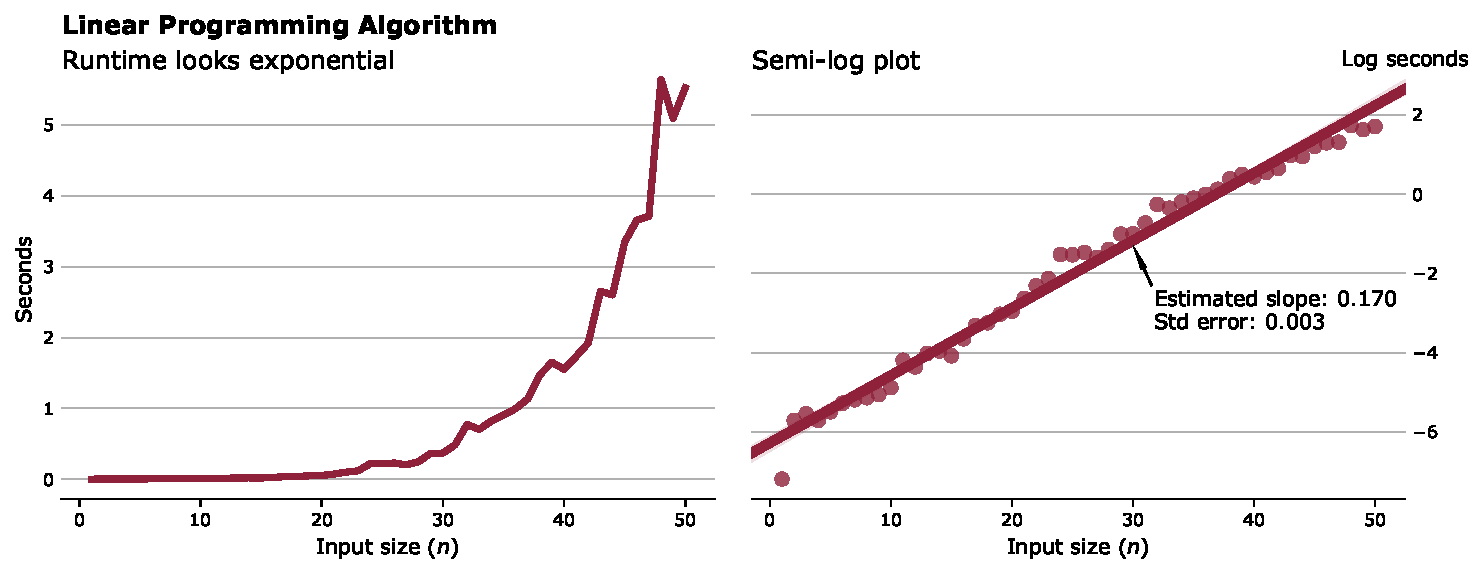
\includegraphics[width=\textwidth]{../../code/lpruntime}
\caption{LP Solver Runtime}
\label{fig:lpruntime}
\end{figure}

We may then benchmark the performance of this data by generating data. We
generate random square $n \times n$ cost matrices by making each entry i.i.d.
$\chi^2(1)$, and perform optimal transport on $\mathbf{a} = \mathbf{b} =
\mathbf{1}_n / n$. The runtimes for different values of $n$ are documented in
\cref{fig:lpruntime}. While this gives us a baseline to how quickly we can
compute optimal transport problems, solving the problem for $n$ bigger than a
couple dozen quickly becomes an expensive task. Thus, we may look elsewhere for
more efficient solutions that either solve a special case or provide an
approximate solution.

% subsection linear_programming (end)

\subsection{Hungarian Algorithm} % (fold)
\label{sub:hungarian_algorithm}

One such special case of the optimal transport problem is when $\mathbf{a} =
\mathbf{b} \propto \mathbf{1}_n$ as in our simulations to test the performance
of the generic LP solver. In this case, mass is being matched in unit pieces,
which makes the problem more tractable. The Hungarian algorithm solves this
special-case. The Hungarian algorithm is also called a dual-ascent method
because it starts by establishing feasible solutions to the primal and dual
problems, and proceeds by improving these solutions until their objectives
match. We empirically test the performance of such an algorithm, providing the
results in \cref{fig:hungarianruntime}. As we can note when comparing to the
general case LP, the run-times for comparably sized problems are distinctly
smaller for the Hungarian algorithm.

\begin{figure}[h]
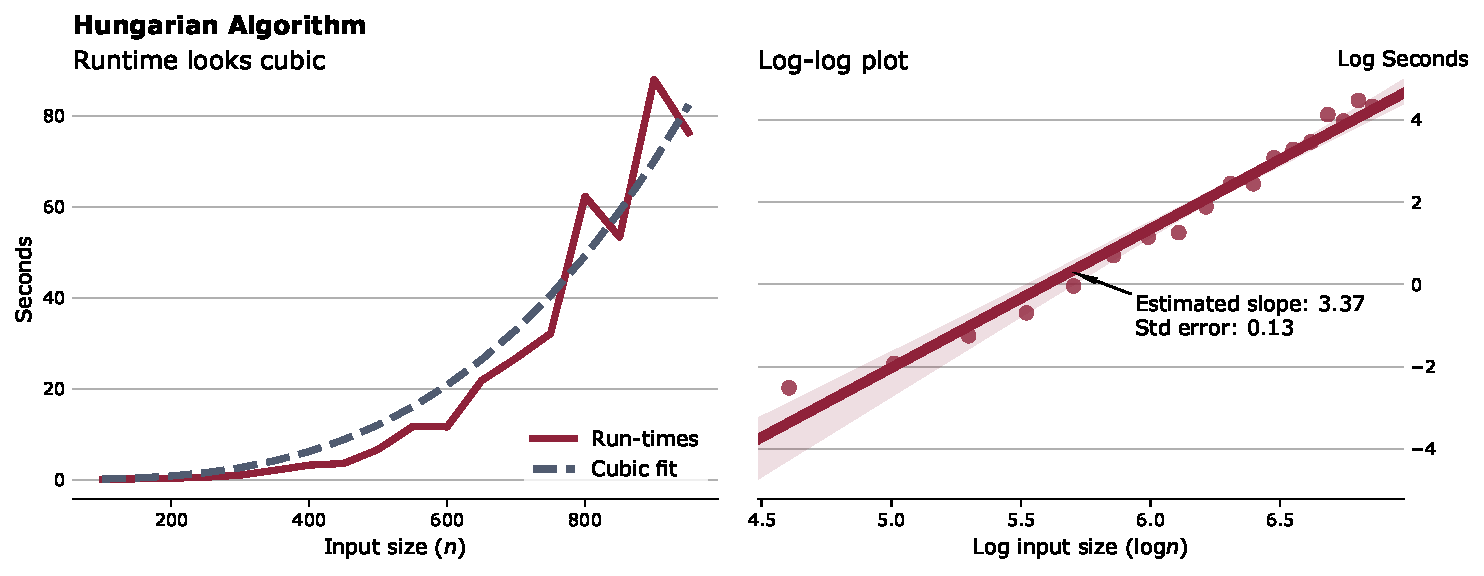
\includegraphics[width=\textwidth]{../../code/hungarianruntime.pdf}
\caption{Hungariant Algorithm runtime}
\label{fig:hungarianruntime}
\end{figure}

% subsection hungarian_algorithm (end)

\section{Inexact Methods} % (fold)
\label{sec:inexact_methods}

\subsection{Entropic Regularization and Sinkhorn's Algorithm} % (fold)
\label{sub:entropic_regularization_and_sinkhorn_s_algorithm}

Let \[H(\b P)= -\sum_{i,j} P_{ij}(\log P_{ij} - 1)\] be the \emph{entropy} of
 the transport matrix $\b P$. Observe that \[
\nabla^2_{\b P} (-H(\b P)) - I \text{ is positive semidefinite},
\]
and so $-H(\b P)$ is 1-strongly convex. We regularize the objective of 
\eqref{eq:ot_problem} by $-\epsilon H(\b P):$ \begin{equation}
\label{eq:entropic}
  \min_{\b P \in \feasible} \sum_{i,j}P_{ij}C_{ij} - \epsilon H(\b P) 
\tag{Entropic Regularization}
\end{equation}
so as to make the objective $\epsilon$-strongly convex. \emph{Entropic
 regularization} approximates \eqref{eq:ot_problem} by solving 
\eqref{eq:entropic}, where \[
\argmin_{\b P \in \feasible} \sum_{i,j}P_{ij}C_{ij} - \epsilon H(\b P) 
 {\underset{n\to\infty}{\longrightarrow}}
 \argmin_{\b P \in \feasible} \sum_{i,j}P_{ij}C_{ij},
\]
where the convergence is towards the maximal-entropy solution of 
\eqref{eq:ot_problem}. The convergence property makes \eqref{eq:entropic} an
 attractive alternative to solving optimal transport; other reasons why 
\eqref{eq:entropic} is useful is explored in a seminal article by 
\cite{cuturi2013sinkhorn}. 

Leveraging duality theory, the Lagrangian of the regularized problem is 
\begin{align*}
\mathcal L(\b P, \b f, \b g) = & \sum_{i,j} P_{ij}C_{ij} + \epsilon \sum_
{i,j} P_{ij}
(\log
 P_{ij} - 1) \\ 
& + \sum_i f_i\pr{a_i - \sum_{j}P_{ij}} + \sum_j g_j \pr{b_j - \sum_i P_{ij}},
\end{align*}
where the first-order condition on $\b P$ shows that the optimum $\b P^\*$
 satisfies 
\begin{equation}
\label{eq:foc}
  C_{ij} + \epsilon \log P_{ij}^\* - f_i^\star - g_j^\* = 0 \implies \b P^\* =
 \diag(\exp(\b f^\* / \epsilon)) \exp(-\b C/\epsilon )\diag(\exp(\b g^\* /
 \epsilon))
\end{equation}
for some $\b f^\star, \b g^\*,$ where the $\exp$ is taken component-wise.
 Suppose $\b f^\star, \b g^\*$ is such that $\b P^\star$ defined by 
\eqref{eq:foc} is within the constraints $\feasible$, then the value of the
 Lagrangian $\mathcal L(\b P^\*, \b f^\*, \b g^\*)$ equals the value of 
\eqref{eq:entropic}, and since  $\b P^\*$ is chosen to maximize the strongly
 concave function $\b P \mapsto \mathcal L(\b P, \b f^\*, \b g^\*)$, we have
 that $(\b P^\*, \b f^\*, \b g^\*)$ solves both programs. 

Before proceeding, we define some notation that is a hybrid of 
\cite{peyre2017computational} and \cite{altschuler2017near}. Let $\b A = \exp
(-\b C / \epsilon),$ $\b u = \exp(\b f / \epsilon)$, $\b v = \exp(\b g /
 \epsilon)$, $\b x = \log \b u$, $\b y = \log \b v$, $\b X = \diag(\b u)$, $\b
 Y = \diag(\b v)$, where $\exp, \log$ are taken componentwise. Thus, we aim to
 find vectors $\b u, \b v$, such that \[
\b P^\* = \b X \b A \b Y.
\]
satisfies the constraints $\feasible.$ In terms of $\b u, \b v$, the constraints
 are \begin{equation}
\label{eq:sinkhorn}
   \b u \odot (\b A \b v) = \b a \quad \text{    and    } \quad \b v \odot (\b A^T
 \b u) = \b b 
 \end{equation}
\eqref{eq:sinkhorn} shows that, given $\b v$, we can only set $\b u = \frac{\b
 a }{\b A \b v}$, where division is componentwise. This motivates the
 Sinkhorn-Knopp algorithm \cite{sinkhorn1967concerning}, which iteratively
 updates
 $\b u, \b v$ such that one of the constraints hold exactly in this fashion. In
 practical implementation, to prevent numerical underflow, the algorithm should
 work in log-space with $\b x, \b y$. \cref{alg:sinkhorn} presents a numerically
 stable implementation of Sinkhorn-Knopp that terminates when the $\ell_1$ error
 on constraint violation gets sufficiently small. At each step of 
\cref{alg:sinkhorn}, if $k$ is odd, then $\b P^{(k)}$ matches row-wise with $\b
 a$, and if $k$ is even, then $\b P^{(k)}$ matches column-wise with $\b
 b$.

\begin{algorithm}
\caption{Numerically stable Sinkhorn-Knopp algorithm as presented in 
\cite{altschuler2017near}}
\label{alg:sinkhorn}

\begin{algorithmic}

\Function{Sinkhorn}{$\b A, \b a, \b b, \epsilon$}
\State Initialize $k=0$
\State $\b P^{(0)} \gets \b A, \b x^0 \gets 0, \b y^0 \gets 0$
\While{$\norm{\b P^{(k)}\one - \b a}_1 + \norm{(\b P^{(k)})^T\one - \b b}_1 >
 \epsilon$}
\State $k\gets k + 1$
\If{$k$ is odd}
\State $\Delta \b x \gets \log\frac{\b a}{\b P^{(k-1)}\one}$
\State $\b x^k \gets \b x^{k-1} + \Delta \b x, \b y^k \gets \b y^{k-1}$
\EndIf
\If{$k$ is even}
\State $\Delta \b y \gets \log\frac{\b b}{(\b P^{(k-1)})^T\one}$
\State $\b x^k \gets \b x^{k-1}, \b y^k \gets \b y^{k-1}  + \Delta \b y$
\EndIf
\State $\b P^{(k)} \gets \b X^k \b A \b Y^{k}$
\EndWhile
\State\Return{$\b P^{(k)} / \norm{\b P^{(k)}}_1$}
\Comment{$\b P^{(0)}$ is not normalized; $\b P^{(k)}, k > 0$ is normalized.}
\EndFunction
\end{algorithmic}
\end{algorithm}

Note that \cref{alg:sinkhorn} does not output a matrix that satisfies the
 conditions $\feasible$ exactly. However, \cite[Algorithm 2]{altschuler2017near}
 analyzes a rounding scheme that forces the output to be inside $\feasible$. The
 rounding scheme introduces error on the order of $\epsilon$ and thus does not
 pose any problems for solving the original program \eqref{eq:entropic}. The
 rest of this section will be devoted to an analysis of \cref{alg:sinkhorn}.

\subsubsection{Convergence}
\emph{A priori}, it is unclear that \cref{alg:sinkhorn} converges, nor is the
 speed of convergence obvious. 
\cite{altschuler2017near} presents an extremely succinct analysis of 
\cref{alg:sinkhorn}, which we reproduce in this section. Let \[
f(\b x, \b y) = \sum_{i,j} A_{ij} e^{x_i + y_j} - \sum_i a_i x_i - \sum_j b_j
 y_j.
\] 
The first order conditions for the optimality of $f$ gives $\b x, \b y$
 that ensures \eqref{eq:sinkhorn}. Sinkhorn-Knopp can be viewed as coordinate
 descent on $f$: To optimize $x_i^k$, the first order condition yields \[
x_i^k = \log \frac{a_i}{\sum_j A_{ij} e^{y_j^{k-1}}} = \log \frac{a_i}{e^
{x_i^{k-1}}\sum_j A_{ij} e^{y_j^{k-1}}} + x_i^{k-1} = \log \frac{a_i}{\b P^{
(k-1)}\one} + x_i^{k-1},
\]
which is exactly the update rule in \cref{alg:sinkhorn}. 

\begin{rmk}
  We do not need to limit ourselves to using coordinate descent to minimize $f$.
 For instance
\cite{brauer2017sinkhorn} uses Newton's method, and achieves similar convergence
 performance as \cref{alg:sinkhorn}.
\end{rmk}

The proof of \cite{altschuler2017near} uses the follow strategy. First, we
 calculate the step gain in the Sinkhorn-Knopp algorithm for optimizing $f$ in
 terms of Kullback-Leibler divergences.
 Next we bound the distance of $f$'s initial value from its optimal value.
 Lastly, using Pinsker's inequality, we show that if \cref{alg:sinkhorn} does
 not terminate, then the step size must be larger than $C\epsilon^{2}$, which
 then gives a bound of convergence in $\epsilon^{-2}$.

For $k > 1$, we can
 calculate the gain of each step \cite[Lemma 2]{altschuler2017near}:
\begin{align}
f(\b x^{k-1}, \b y^{k-1}) - f(\b x^{k}, \b y^{k}) &= \pr{\sum_{i,j} A_{ij}e^
{x_i^{k-1} + y_i^{k-1}} - \sum_{i,j} A_{ij}e^
{x_i^{k} + y_i^{k}}} \nonumber\\&\qquad+ \ip{\b a, \b x^k -\b x^{k-1}} + \ip{\b
 b,
 \b y^k - \b y^{k-1}}
 \nonumber\\
&= (1-1) + \KL(\b a || \b P^{(k)}\one) + \KL(\b b || (\b P^{(k)})^T\one)
 \nonumber \tag{Writing out the inner products}\\
&= \KL(\b a || \b P^{(k)}\one) + \KL(\b b || (\b P^{(k)})^T\one). 
\label{eq:klsum}
\end{align}
\eqref{eq:klsum} gives an elegant formulation of the gain each step exactly as a
 function of the Kullback-Leibler divergence between the target distribution and
 the current marginal distribution.

Next, we claim that the total distance in $f$ that we are required to
 travel is bounded above \cite[Lemma 3]{altschuler2017near}. Note that 
\cref{alg:sinkhorn} behaves almost identically---producing the same $\b P^{(k)}$
 at each iteration---if the input $\b A$ passed in is
 multiplied by a constant. Thus we may without loss of generality replace $\b A$
 with
 $\b A_0 = \b A / \norm{\b A}_1$. Let $f^k$ denote $f(\b x^k, \b y^k)$ and
 $f^\*$ denote $\min f$. Then we have $
f(0,0) - f^1 = \KL(\b a || \b A_0\one) \ge 0.
$
Thus \[
f^1 - f^\* \le f(0,0) - f^\* = \sum_{i} a_i x_i^\* + \sum_j b_j y_j^\* \le \max_
{i,j}
(x_i^\* + y_j^\*).
\]
Observe that $
A_{0, ij}e^{x_i^\* + y_j^\*} \le \sum  A_{0, ij}e^{x_i^\* + y_j^\*} = 1.
$
Therefore $x_i^\* + y_j^\* \le -\log A_{0,ij} \le \log \frac{\norm{\b A}_1}{\min_
{i,j} A_{ij}}$. Putting these together shows that \begin{equation}
\label{eq:total}
  f^1 - f^\* \le \log \frac{\norm{\b A}_1}{\min_
{i,j} A_{ij}}.
\end{equation}

Lastly, Pinsker's inequality \cite[Lemma 4]{altschuler2017near}, a well-known
 result in information theory, states that for any probability measures $p, q$,
 \[
\norm{p-q}_1^2 \le 2 \KL(p||q). 
\]
Applying Pinsker's inequality shows that every step in \cref{alg:sinkhorn}
 before termination has \[
\epsilon < \norm{\b P^{(k)}\one - \b a}_1 + \norm{(\b P^{(k)})^T\one - \b b}_1
 \le \bk{4\pr{\KL(\b a || \b P^{(k)}\one) + \KL(\b b || (\b P^{(k)})^T\one)}}^
{1/2}.
\]
Therefore we improve $f$ by more than $\frac{1}{4}\epsilon^2$ every step before
 termination. Since the total improvement is bounded by \eqref{eq:total}, we
 arrive at the main result of \cite{altschuler2017near}:
\begin{theorem}[\cite{altschuler2017near}]
\label{thm:sinkhorn_convergence}
  \cref{alg:sinkhorn} terminates in at most $4\epsilon^{-2}\log \frac{\norm{\b A}_1}{\min_
{i,j} A_{ij}}$ steps.
\end{theorem}

\begin{figure}[tb]
  \centering
  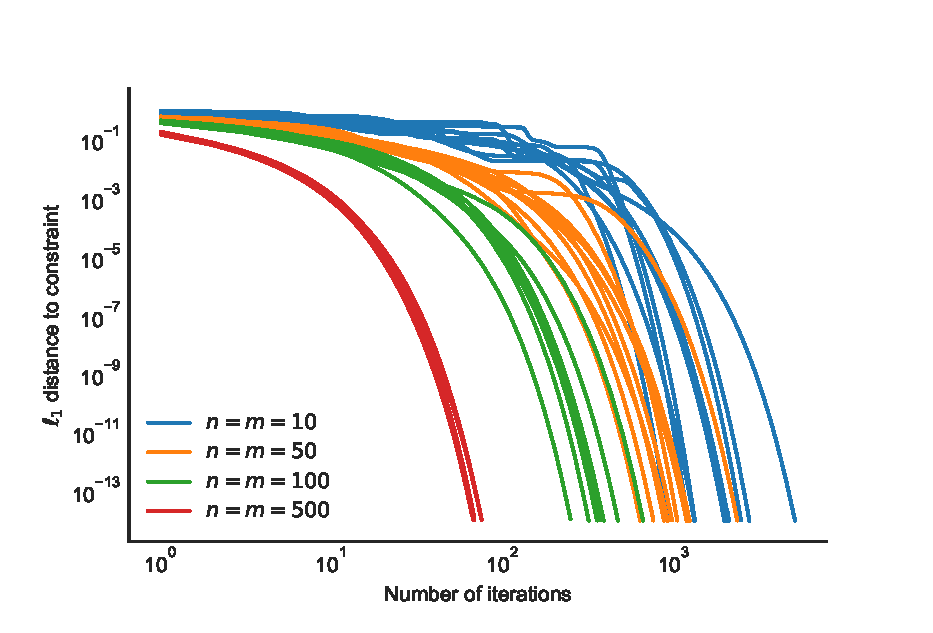
\includegraphics{figs/sinkhorn.eps}
  \caption{Numerical experiments on the speed of $\ell_1$ convergence for \cref{alg:sinkhorn}}
  \label{fig:sinkhorn_convergence}
\end{figure}



\subsubsection{Numerical Experiments}
\label{sub:numerical_sink}
We implement \cref{alg:sinkhorn} and compute the $\ell_1$ distance $\norm{\b P^{
(k)}\one - \b a}_1 + \norm{(\b P^{(k)})^T\one - \b b}_1$ as a function of $k$.
 We generate random marginal distribution targets $\b a, \b b$ by sampling
 from a uniform distribution on the unit interval and normalizing by the sum. We
 generate random cost matrices by sampling each component from a uniform
 distribution. We plot the log-log plot in \cref{fig:sinkhorn_convergence}. Note
 that if the results of \cref{thm:sinkhorn_convergence} is tight for these
 random matrices and constraints, then the log-log plot should look linear with
 slope $-2$. This is not what we observe in \cref{fig:sinkhorn_convergence},
 suggesting that the average case---if not worst case---of \cref{alg:sinkhorn}
 may be better than $O(\epsilon^{-2})$. In fact, if we plot the log of error
 against $k$, we find that the relationship is linear, suggesting that, for these
 random matrices and distributions, the behavior of \cref{alg:sinkhorn} is
 $O(\log(1/\epsilon))$. 

% subsection entropic_regularization_and_sinkhorn_s_algorithm (end)

\subsubsection{Towards a Tightness Analysis of \cref{thm:sinkhorn_convergence}}
\cref{sub:numerical_sink} suggests that the bound of $\epsilon^{-2}$ may be far
 too generous. In this section we sketch a potential direction in analyzing the
 worst-case performance of \cref{alg:sinkhorn}. \cite{sason2015reverse} gives a
 reverse Pinsker's inequality: For discrete probability measures on finite
 support $p,q$, \[
\KL(p||q) \le \log \pr{1+\frac{1}{q_{\min}}\norm{p-q}_1^2} \le \frac{1}{q_{\min}}\norm{p-q}_1^2,
\]
where $q_{\min}$ is the minimum of $q$ on its support. The inequality suggests
 that before termination and after the $\ell_1$ error reaches some $\delta$,
 every
 step of \cref{alg:sinkhorn} improves $f$ by at
 most \[
\KL(\b a || \b P^{(k)}\one) + \KL(\b b || (\b P^{(k)})^T\one) \le \frac{C}
{\min(\b P^{(k)}\one, (\b P^{(k)})^T\one)}\delta^2,
\]
for some constant $C$, where the minimum is taken element-wise. We can remove
 the dependence on $k$ of
 the right-hand side by the following consideration. Let $k'$ be the first time
 that the $\ell_1$-error is below $\frac{1}{2}\min(\b a, \b b)$. Then for every
 $k > k'$, $\min(\b P^{(k)}\one, (\b P^{(k)})^T\one) \ge \frac{1}{2}\min(\b a,
 \b b)$, and so the bound becomes \begin{equation}
   \label{eq:bound_improvement}
\KL(\b a || \b P^{(k)}\one) + \KL(\b b || (\b P^{(k)})^T\one) \le \frac{C'}
{\min(\b a,
 \b b)}\delta^2,
 \end{equation}
for $k > k'$. Let $k_\epsilon$ be the step immediately before termination. Let
 $k_\delta$ be the first iteration such that $k_\delta > k'$ and that $k_\delta$
 reaches $\ell_1$-error of $\delta$.
If we
 can show that there is some inputs $\b A, \b a, \b
 b,\epsilon$ for
 which we can bound the total improvement $f^{k_\eta} - f^{k_\epsilon}$ below by
 some quantity $M(\b A, \b a, \b
 b,\epsilon, \delta)$, then for the inputs $\b A, \b a, \b
 b,\epsilon$, \cref{alg:sinkhorn} has a lower bound of $\Omega\pr{M(\b A, \b a,
 \b
 b,\epsilon, \delta)\delta^{-2}\min(\b a, \b b)}$. Here, $\delta$ should be
 implicitly a function of $\epsilon$, e.g. $\delta = \sqrt{\epsilon}$, so that
 the bound is a function of $\epsilon$. Choosing $\delta(\epsilon)$ such that
 the bound $M(\b A, \b a,
 \b
 b,\epsilon, \delta)$ is tractable is a major difficulty, which we leave to
 future work.


\subsection{Genetic Algorithm} % (fold)
\label{sub:genetic_algorithms_}

Recent advances in machine learning points towards the versatility of genetic
 algorithms, even as a competitive alternative to deep learning based on
 gradient methods \cite{such2017deep}. Inspired by these advances, we consider
 the following genetic algorithm.

\begin{algorithm}
\caption{A toy genetic algorithm for optimal transport}
\label{alg:genetic}

  \begin{algorithmic}
\Function{GeneticOT}{$\phi, \gamma, k, \b a, \b b, T$}
\State $\mathsf{initial} \gets \b a \b b^T$
\State $\mathsf{family} \gets \mathsf{Array}[\phi]$, initialized to $
\mathsf{initial}$
\State $\mathsf{children} \gets \mathsf{Array}[\phi\gamma]$, initialized to
 empty
  \For{$\mathsf{generation}$ in $1:T$}
    \For{$\mathsf{person}$ in $\mathsf{family}$}
      \For{$\mathsf{person}'$ in \Call{Subset}{$\mathsf{family}, \gamma$}} \Comment
{\textsc{Subset} chooses a subset of size $\gamma$}
\State $\mathsf{child} \gets$ \Call{Marry}{$\mathsf{person}, 
\mathsf{person}'$}
\State $\mathsf{child} \gets$ \Call{Perturb}{$\mathsf{child},k$}
\State Add $\mathsf{child}$ to $\mathsf{children}$
\EndFor
\EndFor
\State Choose the $\phi$ elements in $\mathsf{children}$ with minimal cost for
 \eqref{eq:ot_problem} and set to $\mathsf{family}$
\EndFor
\State\Return{element in $\mathsf{family}$ that achieves minimal cost}
\EndFunction
  \end{algorithmic}
\end{algorithm}
Here \textsc{Marry} picks two probability matrices and averages them
 elementwise, and \textsc{Perturb} chooses random indices $i_1,i_2, j_1,j_2$ and
 moves mass in the probability matrix in such a way that preserves the marginal
 distributions and respects the constraint that $0\le p \le 1$ for all
 components $p$. Such perturbations are repeated $k$ times. $\phi$ is a
 parameter that controls the size of families, and $\gamma$ is a parameter that
 decides the number of offsprings. At each generation, we take the top $\phi$
 matrices that achieve the lowest cost. We hoped that the population drifts
 towards the optimal transport matrix as the number of generation increases.

The empirical results we obtain are less than encouraging, however. We plot the
 optimal cost each generation with $n = m = 4, \phi=100, \gamma =5$ for various
 values of $k$ in \cref{fig:genetic_fail}. Curiously, the improvement in the
 first generation is always large, with a magnitude of improvement increasing
 in $k$, but the algorithm seems to achieve some non-optimal steady state as
 generation goes on. Of course, \cref{alg:genetic} can potentially be improved
 by thinking about the design of \textsc{Marry} and \textsc{Perturb} more
 carefully, perhaps leveraging some information about $\b C$. 

\begin{figure}[tb]
  \centering
  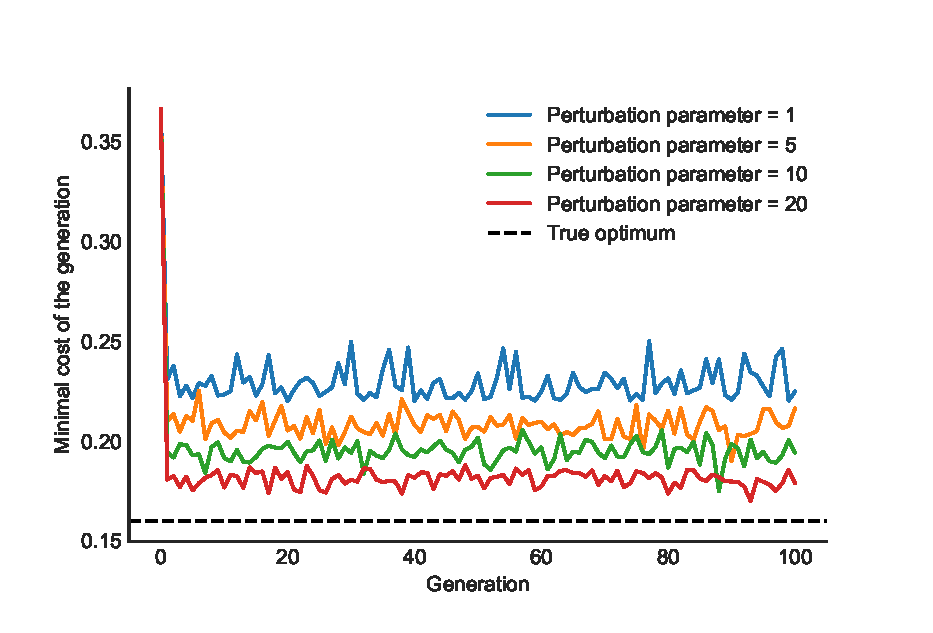
\includegraphics{figs/genetic.eps}
  \caption{Non-convergence of \cref{alg:genetic}}
  \label{fig:genetic_fail}
\end{figure}


% subsection genetic_algorithms_ (end)


\section{Applications and Experiments} % (fold)
\label{sec:applications_}

The applications of the optimal transport problem to the physical transportation
of objects is practically explicit in the problem statement. As we highlight
previously his is but one of many applications. In particular, we explore the
use of optimal transport in the image processing of MNIST images.

\begin{figure}[tb]
  \centering
  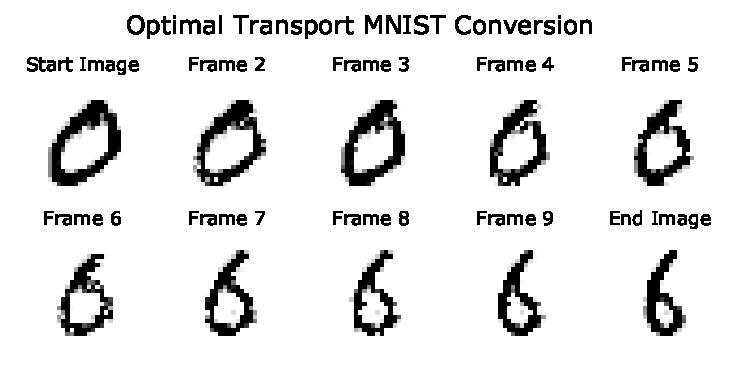
\includegraphics{../../code/ot-mnist-evol.pdf}
  \caption{Optimal transport on MNIST images}
  \label{fig:mnisttransport}
\end{figure}

Optimal transport provides a natural language with which to talk about image
similarity. If we consider the darkness of a pixel as ``mass,''  the similarity
of two images could be quantified as the units of mass times distance that need
to be moved, in order to transform it into the second image. This requires us to
normalize the image such that the pixel intensities sum to 1, but this is not a
problem with MNIST images, which do not differ significantly in their average
brightness. The transport also requires a choice of cost function between two
pixels. We opt for an $L^2$ penalization on the distance between the pixels, but
alternative metrics such as $L^1$ perform similarly. \cref{fig:mnisttransport}
illustrates what this transformation looks like for a ``0'' being transported
into a ``6.'' 

To verify that the similarity is behaving as we expect, we can compare the
similarity of a number ``5'' against its most similar images in a small sample
of the MNIST dataset. The most similar images are also 5's, as depicted in
\cref{fig:mnistsim}.


\begin{figure}[tb]
  \centering
  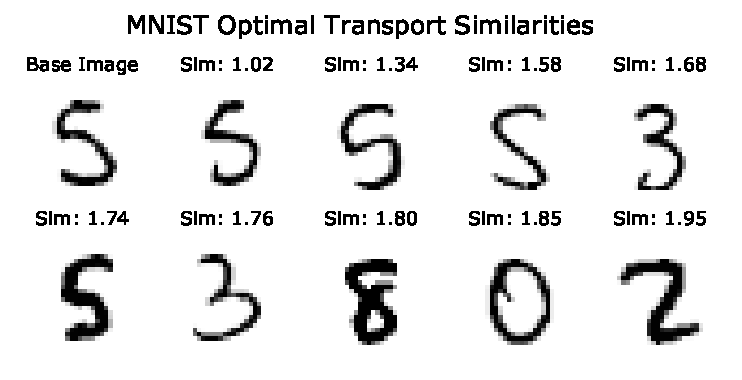
\includegraphics{../../code/mnist-similarity.pdf}
  \caption{MNIST Similarity Metric}
  \label{fig:mnistsim}
\end{figure}




\section{Conclusion} % (fold)
\label{sec:conclusion}

To conclude, our goals in surveying the topics presented are two-fold. Firstly,
we hope to illustrate the richness of the computational toolkit appropriate for
solving optimal transport problems. We survey both exact methods, such as the LP
formulation and the Hungarian method, as well as potentially faster inexact
approximations, such as the \eqref{eq:entropic} problem and genetic algorithms.
In doing so, we emphasize both theory and empirics to understand how these
algorithms perform from different perspectives.

Second, we hope to convey the flexible applicability of the optimal transport
problem. We illustrate this with a foray into machine vision and the MNIST
dataset as well as motivation of different intuitions for the optimal transport
problem.


\bibliographystyle{alpha}
\bibliography{../optimal-transport}
\end{document}
